\documentclass[11pt,a4paper]{article}
\usepackage[margin=1in]{geometry}
\usepackage[T1]{fontenc}
\usepackage[utf8]{inputenc}
\usepackage{graphicx}
\usepackage{setspace}
\usepackage{parskip}
\usepackage{titlesec}

\setstretch{1.02}
\pagenumbering{gobble}
\titleformat{\section}{\normalsize\bfseries}{}{0em}{}

\begin{document}

\begin{center}
{\Large A Brief Note on the U.S. Output Gap, 1990--2020}
\end{center}

Figure 1 plots the quarterly U.S. output gap from 1990 to 2020, computed as the percentage difference between real GDP and CBO potential GDP. Positive values indicate that realized output was above estimated potential, while negative values indicate economic slack. Over the sample, the series displays a familiar cyclical pattern: moderate weakness in the early 1990s, persistent strength in the second half of that decade, a mild deterioration in the early 2000s, a deep contraction during the Global Financial Crisis, and an extraordinary collapse in 2020 with the onset of the pandemic.

At the beginning of the sample, the output gap turns negative during the 1990--1991 recession. The decline is not dramatic by historical standards, but it signals a period in which aggregate demand was insufficient to keep actual production aligned with the economy's productive capacity. The gap then narrows gradually during the recovery and becomes clearly positive in the second half of the 1990s. This episode is consistent with the strong productivity growth, robust investment, and buoyant labor market conditions that characterized the expansion of that period. By the turn of the millennium, the economy appears to have been operating above potential for several years.

The early-2000s slowdown reduces the gap, but the series remains relatively close to zero compared with later episodes. The major break in the figure is the 2008--2009 recession: the output gap falls sharply and stays deeply negative for several years. This persistence is important because it suggests that the recovery was long but incomplete, with actual GDP recovering more slowly than potential output. Through much of the 2010s the gap gradually closes, and by the end of the decade the economy again fluctuates near potential, without showing the sustained overheating seen in the late 1990s.

The final observation is the most striking. In 2020 the output gap plunges abruptly as real activity collapses in response to the COVID-19 shock. Relative to earlier downturns, the pandemic recession is distinguished by both its speed and magnitude. Even though output rebounds quickly after the second quarter of 2020, the series remains clearly negative by the end of the sample, indicating that the recovery was still incomplete. Overall, the figure summarizes the cyclical history of the U.S. economy over three decades and highlights how estimates of slack can help compare recessions not only by depth, but also by the persistence of the return toward potential.

\begin{center}
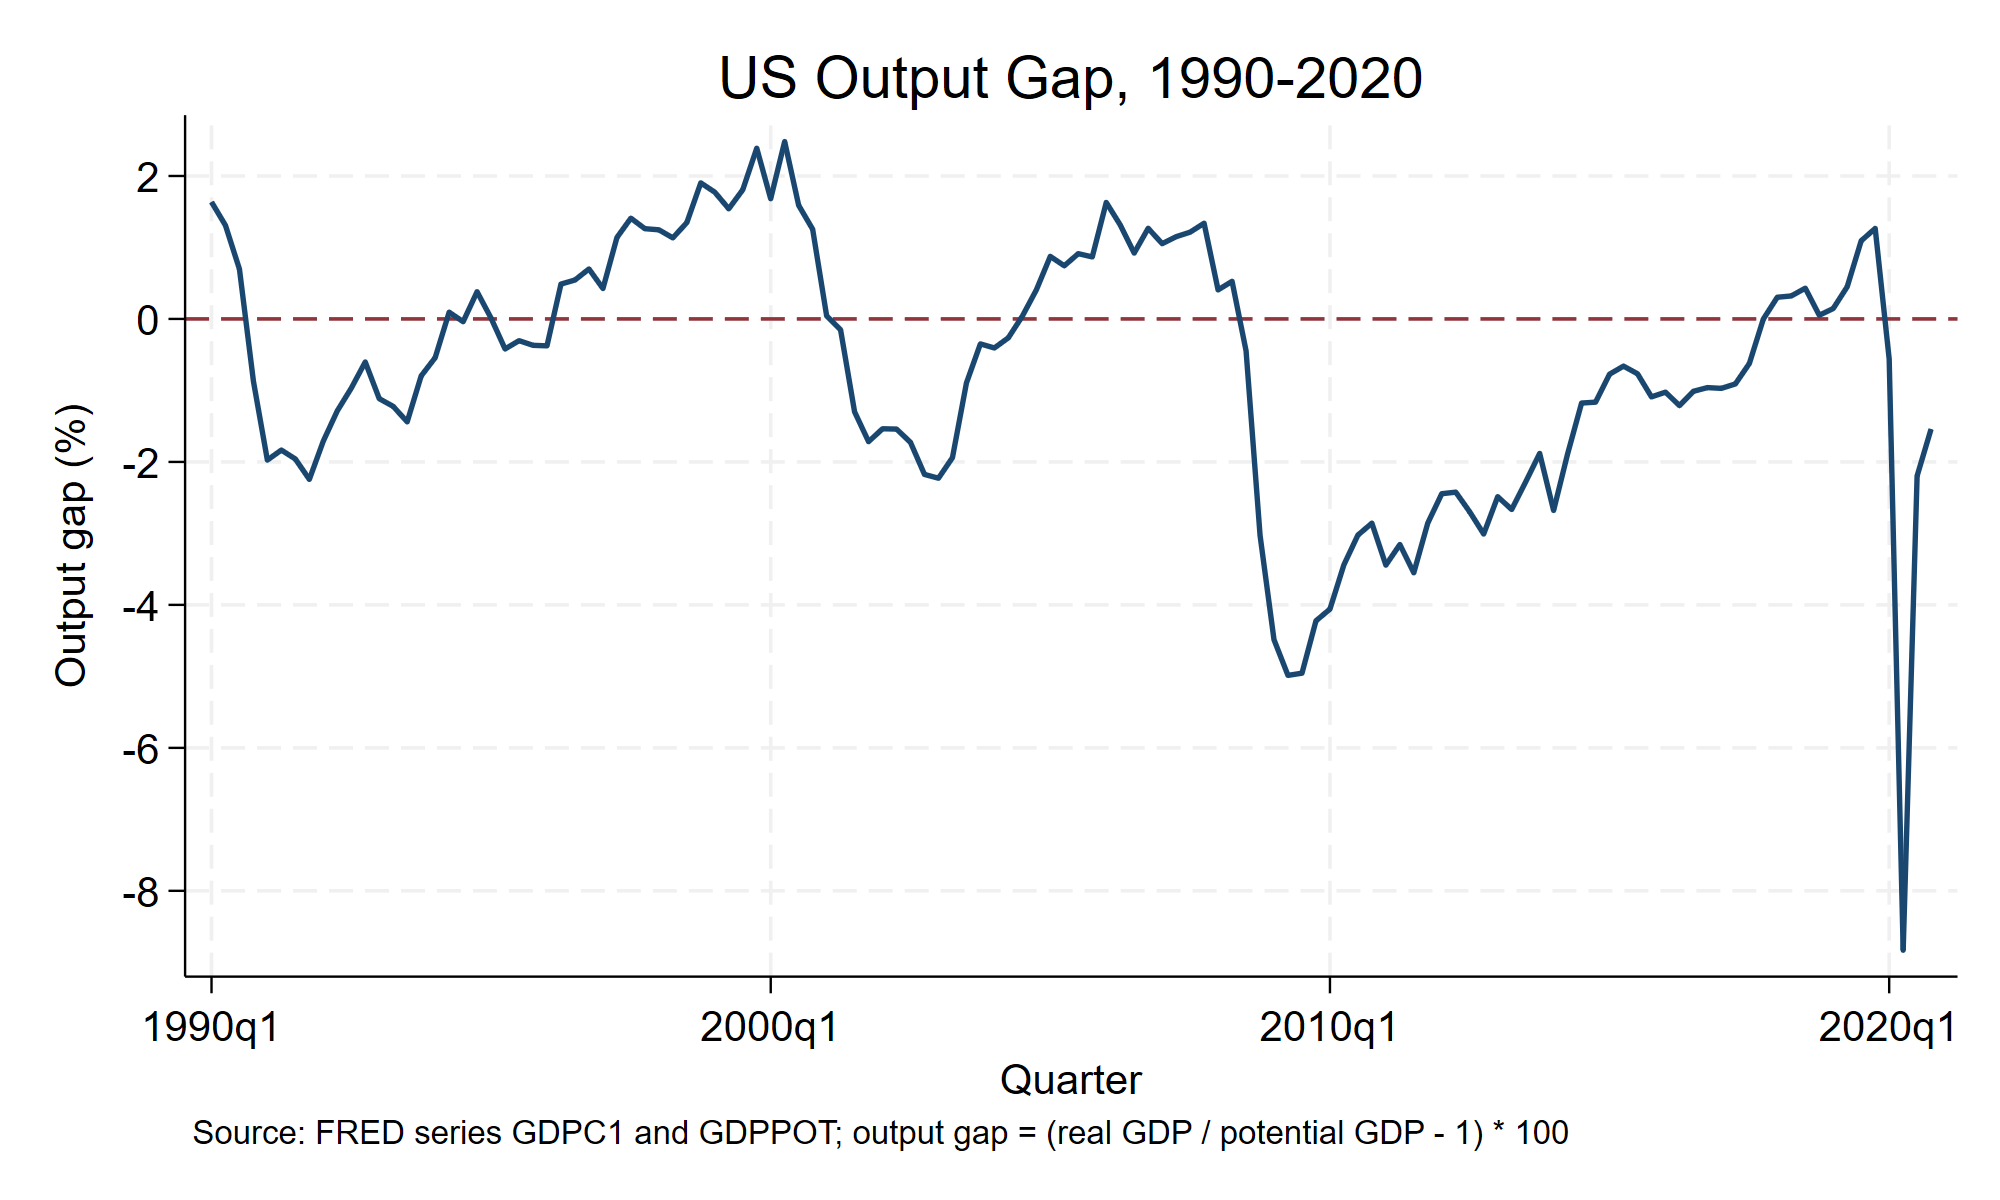
\includegraphics[width=0.9\textwidth]{data/us_output_gap_1990_2020_quarterly.png}

\small Figure 1. U.S. output gap, quarterly data, 1990--2020.
\end{center}

\end{document}
